% !TEX TS-program = XeLaTeX
\documentclass{CSICC2020}

% تقریبا تمامی بسته‌های مورد نیاز برای یک مقاله در استایل فراخوانی شده است. اما در هر صورت در صورتی‌که می‌خواهید بسته‌ای را فراخوانی کنید به صورت زیر عمل کنید. مثلا ما در کد زیر دوبسته glossaries و tikz را فراخوانی کرده‌ایم.
%\makeatletter
%\bidi@BeforePackage{xepersian}{
%\RequirePackage{tikz}
%\RequirePackage{glossaries}
%}
%\makeatother


% عنوان مقاله را در این قسمت وارد کنید. 
\title{
\lr{Overview on Composable UI}

نگاهی کلی به رابط کاربری ساختنی
}
\date{1399/04/18}
% اسامی نویسندگان و همچنین اطلاعات مربوط به آن‌ها را در این قسمت وارد کنید. 
\author[1]{حسین خادمیان}
\affil[1]{
دانشجوی کارشناسی، مهندسی کامپیوتر، دانشگاه شیراز ، شیراز،
me@hkhademia.ir
}


\begin{document}
\maketitle
\begin{abstract}
در این مقاله، به معرفی روابط کاربری Composible ، مزایا و معایب این سیستم، علت چرخش شرکت های بزرگ فناوری به استفاده از این شیوه ساخت روابط کاربری و همچنین نگاه و طریقه آنها در پیاده سازی می پردازیم.
 \end{abstract}
\begin{keywords}
\lr{UI, Composable UI, Flutter, Jetpack Compose, Swift UI, React JS, React Native.}
\end{keywords}

\section{مقدمه}
شیوه کنونی تولید روابط کاربری بر مبنای تعریف عناصر صفحه صفحه نمایش به صورت اشیایی شناخته شده و با جداسازی \lr{widget} های گوناگون مانند \lr{Button}، \lr{ListView}، \lr{DropBox}، \lr{CheckBox}، ... استوار است.

این شیوه توصیف لایه های کاربری در پلتفرم های گوناگون، جهت پیاده سازی رابط کاربری برنامه ها در سیستم عامل ها دستگاه های مختلف (از جمله کامپیوتر شخصی، تبلت، موبایل، صفحات وب و ...) پیاده سازی می شد.


\section{تکنولوژی های پیشین}
\label{History}
جهت پرداختن به مزایا و معایب لایه های کاربری ساختنی و همچنین برسی تفاوت های آن با شیوه های پیاده سازی کنونی ابتدا باید آشنایی کلی با وضعیت فعلی داشته باشیم.
در ادامه به معرفی چند مورد از شیوه های پر استفاده که با آنها کار کرده ام جهت بررسی میپردازم:

\subsection{\lr{HTML} در صفحات وب}
\label{HTML}
صفحات وب مجموعه ای از المنت هاست
\LTRfootnote{read more : \href{https://en.wikipedia.org/wiki/HTML}{HTML}}
که هرکدام مشخص کننده قسمتی از ویژگی های صفحه درحال نمایش هستند. صفحات وب از چندین تگ کلی:
\begin{enumerate} 
\item \lr{<HTML>}: این تگ در برگیرنده کل اطلاعات صفحه است
\item \lr{<BODY>}: این تگ در برگیرنده کل محتوای قابل نمایش صفحه است
\item \lr{<HEAD>}: در این بخش اطلاعات صفحه مانند عنوان و استایل صفحه معرفی می شوند
\end{enumerate} 

\begin{figure}
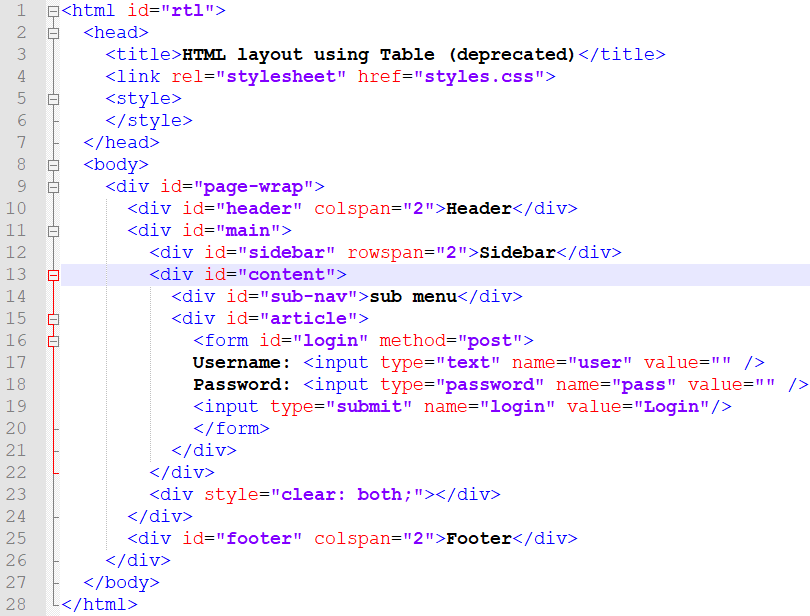
\includegraphics[width=\linewidth]{Images/html}
\caption{نمونه کد \lr{HTML}}
\label{fig:HTML}
\end{figure}

از خواص این نوع تعریف لایه کاربری: تعریف قسمت های مختلف صفحه (دکمه ها، فرم ها، زیرصفحه و ...) در کنار مشخصات و ویژگی های آنها (رنگ، فونت، ...) و حتی کد های رویداد های مختلف در کنار هم است.

{\bf مزایا: }
\begin{enumerate} 
\item این مدل توصیفی است، یعنی برنامه نویسی بدون نیاز به کد نویسی به توصیف لایه کاربری می پردازد.
\item زبان ساده و خوانا، قابل استفاده برای نا-برنامه نویسان (طراحان، دانش آموزان و ...)
\LTRfootnote{See also: \href{https://medium.com/@switchweb52/7-benefits-of-html-for-websites-f56ef2e13d5e}{Pros of HTML}}
\item چشم پوشی از خطا: اگر در توصیف لایه کاربری خطایی (در بارگزاری یا حتی سمت برنامه نویس) رخ دهد کل برنامه بی استفاده نمی شود.
\LTRfootnote{See also: \href{https://www.techwalla.com/articles/the-disadvantages-of-html}{Cons of HTML}}
\end{enumerate} 

{\bf معایب:}
\begin{enumerate} 
\item فقط امکان تولید صفحات استاتیک به تنهایی دارد
\item مخلوطی از تمامی منطق برنامه، ظاهر کاربری، کنترل و اطلاعات. باعث عدم امکان توسعه خطی در پروژه های بزرگ و سازمانی می شود.
\item نیازمند دیگر ابزار جهت پویا سازی مثل جاوااسکریپت، activeX و ...
\item صاحب و مدیر StateMachine است و برنامه نویس فقط با event ها از تغییرات وضعیت با خبر می شود. و کنترل کاملی روی آن ندارد. این مسئله باعث به وقوع پیوستن nonDeterministic States می شود.
\end{enumerate} 

\subsection{\lr{WindowsForms, UWP, WPF}}
\label{WindowsForms}
پلتفرم WindowsForms تکنولوژی قدیمی بر بستر WindowsAPI ارایه می شود و به طور کلی ابزاری جهت پیاده سازی رابط کاربری گرافیکی برای برنامه های ویندوزی (GUI) است.
در این پلتفرم جهت توصیف لایه کاربری مستقیما با LayoutEditor نسبت به تعریف رابط کاربری اقدام می کنیم.
ایده پشت این پلتفرم Form-Based بودن است. به این شیوه که تمامی صفحاتی که کاربر با آن تعامل می کند در حقیقت فرمی جهت ورود اطلاعات و دریافت بازخورد از اوست.

\begin{figure}
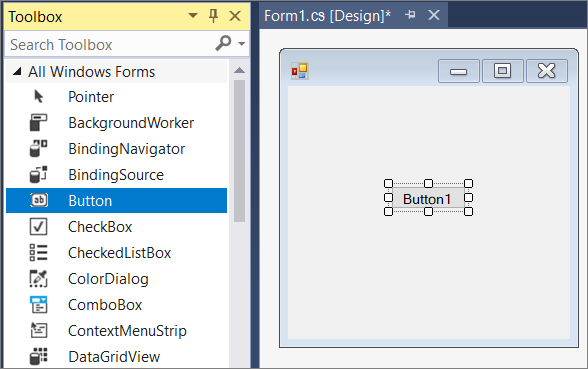
\includegraphics[width=\linewidth]{Images/winform}
\caption{نمونه طراحی با ویرایشگر \lr{WinForm}}
\label{fig:WinForm}
\end{figure}

نسخه بروزتر از این پلتفرم UWP و WPF که به ترتیب برای توسعه برنامه های چند سکویی و دسکتاپ طراحی شده اند دارای زبانی جهت توصیف لایه کاربری به نام XAML هستند.
 این شیوه شباهت بسیاری به ضفحات HTML داشته و بیشتر مزایا و معایب آن در این شیوه هم صادق است.

\begin{figure}
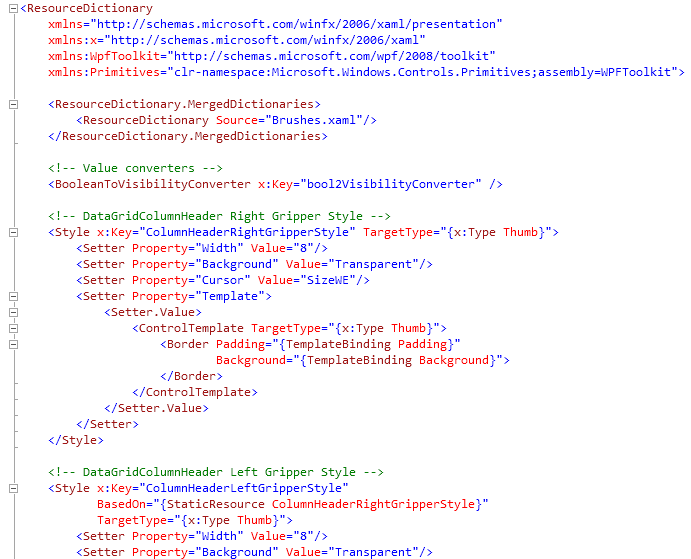
\includegraphics[width=\linewidth]{Images/xaml}
\caption{نمونه کد \lr{XAML}}
\label{fig:XAML}
\end{figure}

\section{زمینه}
\label{Context}
تا کنون با تعدادی از شیوه های تولید رابط کاربری قدیمی آشنا شدیم. در اکثر این شیوه ها برنامه نویس هیچ گونه مدیریتی بر وضعیت ماشین (برنامه) و محتوای نمایش داده شده به کاربر به طور مستقیم ندارد. بلکه با استفاده از ویجت های ارایه شده هر پلتفرم و با اتکا به رویداد های گزارش شده آنها به بروزرسانی وضعیت مد نظر می پردازد.

این شیوه از مدیریت وضعیت و اتکا به پلتفرم های گوناگون (با امکان آپدیت و تغییرات) باعث مشکلات بسیاری در برنامه ها می شود.

اکثر ما تا کنون با برنامه هایی که برخلاف انتظار برنامه نویس به وضعیتی نامطلوب رفته اند (فرضا یک دیالوگ "درحال بارگزاری" در یک برنامه اندرویدی که با چرخش صفحه ناپدید می شود اما از دید برنامه هنوز باید نمایش داده می شد). یکی از مهمترین دلایل این تجارب، نه از عدم آگاهی توسعه دهنده بلکه از {\bf غیر قابل پیش بینی بودن پلتفرم} ایجاد می شود.

جهت مدیریت اینگونه وضعیت های از قبل پیشبینی نشده که اکثرا به علت نقص در پلتفرم، بروز نبودن پلتفرم در دستگاه کاربر (مثل نسخه اندرویدی دستگاه)، عدم شناخت کافی توسعه دهنده از ویژگی ها و عکس العمل های هر کامپوننت در شرایط گوناگون نشات می گیرد، مستلزم به بکارگیری تیم آزمایش محصول و همچنین فرایند پیچیده تر دریافت گزارش های خطا از کاربر می شود. 
حتی گاهی مدیریت یک وضعیت ناخواسته از خود منطق برنامه پیچیدگی بیشتری پیدا میکند.

\begin{figure}

\includegraphics[width=\linewidth]{Images/loading}
\caption{نمونه دیالوگ درحال بارگذاری قبل از چرخش}
\label{fig:Loading}
\end{figure}

یکی دیگر از موارد مهم، Reusability کد ها و کامپوننت هایی که یک برنامه نویس تولید و استفاده می کند است. در شیوه سنتی به دلیل وابستگی کامل برنامه نویس به زمینه ای که در آن یک کامپوننت نوشته می شود (از جمله موقعیت قرار گیری در صفحه، المنت های دیگر صفحه و ...) امکان استفاده از یک کامپوننت در دیگر جاهای برنامه کمتر و فرایند آماده سازی یک کامپوننت برای استفاده در پروژه های دیگر خیلی هزینه زیادی دارد.

اکثر مشکلات اشاره شده در این قسمت و قسمت های قبل از عدم کنترل برنامه نویس بر وضعیت کنونی برنامه و همچنین متمرکز نبودن مرجعیت درستی وضعیت در کل برنامه است. 
برای مثال: به این صورت که از دید برنامه نویس چک باکس شماره 1 فعال و چک باکس 2 غیر فعال است. با تغییر این انتخاب توسط کاربر در اکثر پلتفرم ها ابتدا وضعیت تغیر پیدا کرده و سپس تغییر جدید به برنامه نویس از طریق Event ها اطلاع داده می شود. و برنامه نویس کنترلی روی این تغییر ندارد.

\section{راه کار}

راه حل این مسئله فرستادن کل فرایند رسیدیگی و مدیریت وضعیت ها به برنامه نویس و رندرینگ و ... به پلتفرم است.
همچنین کامپوننت های تشکیل دهنده لایه کاربری هیچ گونه وضعیتی آشکار (قابل مدیریت توسط برنامه نویس) نگه داری نکنند. به این ترتیب حتی تغییر وضعیت یک دکمه رادیویی، تایپ در یک تکست باکس هم با اطلاع و موافقت برنامه نویس صورت میگیرد.

برای پیاده سازی این شیوه تولید کامپوننت های لایه کاربری نیاز است که تغییری در نحوه نگاه به لایه های کاربری به طور کلی بیاندازیم. از جمله:

\begin{enumerate} 
\item هر کامپوننت فقط باید به نقش انحصاری خود بپردازد و در کار بقیه قسمت ها تغییری ایجاد نکند.
\item اطلاعات مورد نیاز جهت پیاده سازی به کامپوننت به آن داده می شود. همچنین کامپوننت از هرگونه تغییری در اطلاعات باید آگاه شود.
\item کامپوننت ممکن است جهت اجرای نقش مشخص شده خود، دارای وضعیتی داخلی باشد که البته هیچ تاثیری در وضعیت کلی برنامه نباید بگذارد.
\item کامپوننت ها نباید وابستگی به والد یا فرزندان خود داشته باشند و به تنهایی و در هر محیط و usecase بتوانند وظیفه مربوطه را انجام دهند.
\end{enumerate}

یکی از دیدگاه های مفید در این زمینه به این صورت مطرح میشود که:

\lr{UI is a function of State}

به این معنی که هرگونه تغییر در وضعیت برنامه در ظاهر کاربری اثر میگذارد و نه برعکس.
ظاهر کاربری هیچگونه مسیولیتی در زمینه صحت سنجی، بروز رسانی، مدیریت، بارگذاری و پردازش اطلاعات ورودی و خروجی و همچنین وضعیت فعلی برنامه ندارد و تنها مسئولیت آن به نمایش گذاشتن وضعیت فعلی اطلاعات برنامه است.

در ادامه چندین پیاده سازی این راه کار را بررسی می کنیم:


\subsection{ویژگی متن اصلی مقاله}
متن اصلی مقاله خود می‌تواند در چهار بخش مختلف دسته‌بندی شود. 
\subsubsection{ویژگی‌های بخش پیش‌نیازها}
در صورتی‌که نویسندگان لازم است که یک مطلب را برای خوانندگان به عنوان پیش‌نیاز و پیش‌زمینه فهم روش پیشنهادی خود ارایه کنند این موارد را در این بخش می‌توانند بیاورند. به عنوان مثال اگر شما می‌خواهید یک روش مبتنی بر یادگیری \lr{SVM} در حوزه نهان‌کاوی تصویر ارایه دهید، می‌توانید توضیحات مقدماتی در مورد \lr{SVM} را در این بخش بیان کنید. البته توصیه کلی بر این است که در حد امکان از آوردن مطالبی که خواننده می‌تواند آن را براحتی با خواندن مراجع دیگر بدست آورد، پرهیز کنید.
\subsubsection{ویژگی‌های بخش مدل سامانه و فرضیات}
در این بخش نویسندگان باید مدل سامانه را به صورت دقیق مشخص کنند. اگر سامانه مورد بررسی و یا کار آن‌ها دارای فرضیات مشخصی است باید آن را در این قسمت مشخص کنند. شما باید سامانه را به‌گونه ای مدل کنید و فرضیات را به نحوی تعیین کنید که چندان به دور از ذهن و بدور از مدل‌ها و فرضیات مقالات گذشته نباشد.



\subsubsection{ویژگی بخش روش پیشنهادی}
\label{Sec:TheProposedMethod}
در این بخش شما باید  به دقت و گام به گام به معرفی کار انجام شده و نوآوری صورت‌گرفته در مقاله مبادرت بورزید. 

برای وارد کردن الگوریتم و سودو کد از محیط \lr{algorithm} استفاده کنید. 
\begin{algorithm}[t]
\caption{الگوریتم ثبت تصویر لوکاس-کاناد مبتنی بر بهینه‌سازی گوس-نیوتون \lr{(LK-GN)}.}
\label{alg1}
\begin{latin}
\textbf{Input}:
The reference image $I$ and template image $T$.\\
\textbf{Output}: Registration parameters
$\mathbf{p}=(p_1,\dots,p_n)^T$ as the warp model $W$.
\begin{algorithmic}[1]
\REPEAT
  \STATE Warp $I$ with $W$ to compute $IW$. 
  \STATE Compute the error image $T(x)-IW$ 
  \STATE Warp the gradient $\nabla I$ with $W$. \STATE Evaluate the Jacobian
    ${W}{p}$ at $(\mathbf{x;p})$. 
  \STATE Compute the steepest descent images $\nabla I{W}{p}$. 
\LOOP \STATE{<text>} \ENDLOOP
  \STATE \label{line:Hessian} Compute the Hessian matrix using   \eqref{eq:dols}. 
\FOR{<condition> \TO <condition> } \STATE{<text>} \ENDFOR
 \WHILE{<condition>} \STATE{<text>} \ENDWHILE
  \STATE \label{alg1:deltap} Compute $\triangle\mathbf{p}$ using \eqref{eq:sams} 
\RETURN Update the parameters $\mathbf{p}\leftarrow\mathbf{p}+\triangle\mathbf{p}$ 
\UNTIL{$||\triangle\mathbf{p}||\leq\epsilon$ or Reaching to Maximum Iteration allowed}
\end{algorithmic}
\end{latin}
\end{algorithm}
توصیه می‌شود که نویسندگان حتما سعی کنند روش خود را به صورت شماتیک با یک فلوچارت و یا استفاده از محیط الگوریتم نمایش دهند. نمونه‌ای از فلوچارت نیز در شکل \ref{fig:OneLRoneHR} نشان داده شده است. دقت کنید که در وارد کردن هرگونه تصویری در مقاله از قرار دادن \lr{option} هایی به مانند
\lr{H}، \lr{!ht} و ...
خودداری کنید. نویسندگان دقت داشته‌باشند که می‌بایست روش پیشنهادی خود را به صورت ساده، واضح و مشخص بیان کنند. سعی کنید در این بخش روش پیشنهادی را در حالت کلی مورد بررسی قرار دهید، و سپس در بخش‌های بعدی به جوانب آن بپردازید. اگر روش پیشنهادی شما دارای چندین مرحله (فاز) است، بهتر است هر مرحله را در یک زیربخش به صورت مجزا مورد بررسی قرار دهید.


\begin{figure}

\includegraphics[width=.9\linewidth]{Images/blank}
\caption{چارچوب کلی روش پیشنهادی.}
\label{fig:OneLRoneHR}
\end{figure}


\subsubsection{ویژگی‌های بخش تحلیل و ارزیابی}
در صورتی که روش پیشنهادی حسی نبوده ومبتنی بر استدلال ریاضیاتی باشد، می‌توان به ارزیابی عملکرد آن در سامانه و نحوه بهبود نتایج نسبت به کارهای گذشته به طور کمی و کیفی پرداخت. بدیهی است اگر مدل پیشنهادی حسی بوده و قابل استناد ریاضیاتی نباشد، تنها می‌توان به صورت کیفی به ارزیابی عملکرد پرداخت.


\subsection{ویژگی‌های بخش شبیه‌سازی}
\label{Sec:ExperimentalResults}

از آنجایی که بسیاری از تحقیق‌ها به منظور حل‌مساله‌ای عملی پی‌گیری می‌شوند، این بخش از اهمیت خاصی برخوردار است. در این بخش به معرفی شبیه‌سازی صورت گرفته و ارائه نتایج به صورت مطلوب (جدول، نمودار و ...) پرداخته می‌شود. در مواردی که طرح پیشنهادی اثبات شده است، نتایج باید با تقریب خوبی با مدعا یکسان باشد. در مواردی که طرح پیشنهادی اثبات نشده و به طور حسی و مبتنی بر برخی پیش‌فرض‌ها مطرح شده است،  اهمیت این بخش بیشتر از حالت قبل است، چرا که نتایج شبیه‌سازی تنها مستند نویسنده و به نوعی موید مدعای ثابت نشده وی است. این حالت اخیر از دهه آخر قرن بیستم تا کنون به وفور در مقالات معتبر پی‌گیری شده است تا جایی که در صورت تایید نتایج با شبیه‌سازی، آن را به نوعی اثبات برای طرح پیشنهادی در نظر می‌گیرند.

\begin{figure}

\includegraphics[width=.9\linewidth]{Images/blank}
\caption{
زیرنویس نمودارها باید کامل و جامع باشد، به عبارت‌دیگر خواننده بتواند با دیدن نمودار و خواندن زیرنویس آن پی به تمامی اطلاعات نهفته در نمودار ببرد.}
\label{fig:sumXYPlot}
\end{figure}
برای آوردن اشکال در کنار یکدیگر می‌توانید از محیط \lr{subfigure} استفاده کنید. 
\begin{figure*}
\centering
\begin{subfigure}[b]{0.31\textwidth}

\includegraphics[width=\linewidth]{./Images/blank}
\caption{}
\label{fig:gull}
\end{subfigure}
\begin{subfigure}[b]{0.31\textwidth}

\includegraphics[width=\linewidth]{./Images/blank}
\caption{}
\label{fig:tiger}
\end{subfigure}
\begin{subfigure}[b]{0.31\textwidth}

\includegraphics[width=\linewidth]{./Images/blank}
\caption{}
\label{fig:EntropyVersus}
\end{subfigure}
\caption{
آ) این شکل در این مورد سخن می‌گوید که .....، ب) در مورد این شکل اکنون صحبت کنید... ، ج) این شکل برای ....
}
\label{fig:animals}
\end{figure*}
در شبیه‌سازی‌ها می‌بایست نویسندگان به صورت دقیق و صریح پیکربندی شبیه‌سازی و مجموعه داده‌ای که مورد استفاده قرار داده‌اند را با ذکر منابع و مراجع مورد نیاز، ذکر کنند. در ضمن پارامترهای مورد استفاده برای شبیه‌سازی باید در همین بخش شبیه‌سازی تعریف شود. به عنوان مثال اگر شما از پارامتر 
\lr{MSE (mean squared error)}
استفاده می‌کنید باید آن را در این بخش تعریف کنید. شکل‌های شبیه‌سازی باید واضح و مشخص باشد. دقت کنید به دلیل این‌که در نهایت مقالات پذیرفته شده به صورت سیاه و سفید چاپ خواهد شد، بدین‌سان از تمایزگذاری با رنگ‌های مختلف بین نمودارها کافی نخواهد بود. یک نمونه از تمایزگذاری مناسب را می‌توانید در نمودار \ref{fig:sumXYPlot} و \ref{fig:tiger} ملاحظه کنید. 

تمامی نمودارهای قسمت شبیه‌سازی باید دارای  \lr{Legend} باشند. محور‌های نمودارها همگی باید دارای برچسب مناسب و همچنین شماره‌گذاری مناسب باشد. در \lr{\LaTeX} سعی کنید نمودارهای خود را با کیفیت \lr{pdf} وارد کنید و از قراردادن نمودارهای  با کیفیت \lr{jpg} و یا کیفیت تصویری خودداری کنید. بسیاری از ابزارهای شبیه‌سازی به شما خروجی \lr{pdf}  را می‌دهند. 

استفاده از نمودارهای نوین به مانند \lr{Box-Plot} به شدت مورد استقبال قرار می‌گیرد. نکته مهم در شبیه‌سازی
انجام پذیرفته در مقاله این است که نویسندگان تنها به گزارش میانگین خطا بسنده کرده‌اند. از دیدگاه علم شبیه‌سازی این کار نمی تواند اطمینان خواننده را به شبیه‌سازی جلب کند. به عنوان مثال دو کلاس را در نظر بگیرید که نمرات سه دانشجوی آن ۹، ۱۰ و ۱۱ است و کلاس دیگر ۵، ۱۰ و ۱۵. هر دو کلاس میانگین یکسانی دارند، اما واقعا بین نمرات این دو کلاس تفاوت زیادی وجود دارد. به عنوان پیشنهاد می توانید از نمودار
\href{https://en.wikipedia.org/wiki/Box_plot}{Box-Plot}
استفاده کنید و یا حداقل بازه اطمینان نتایج را گزارش کنید. نمونه ای از یک \lr{Box-Plot} در شکل
\ref{fig:EntropyVersus}
نشان داده شده است. 

سعی کنید از قرار دادن کدهای شبیه‌سازی چه در قسمت شبیه‌سازی و چه در قسمت روش پیشنهادی به شدت خودداری کنید. نویسندگان به صورت اختیاری می‌توانند کدهای شبیه‌سازی خود را در یک وب‌سایت قرار داده و به آن در مقاله پیوند دهند. 

\subsection{ویژگی‌های بخش نتیجه‌گیری}
در بخش نتيجه، نكات مهم انجام شده در كار بصورت خلاصه مرور و نتايج به دست آمده توضيح داده شوند. همچنين در اين بخش بايد سهم علمي مقاله بصورت واضح بيان شود. هرگز عين مطالب چكيده را در اين بخش تكرار نكنيد. نتيجه می‏‌تواند به کاربردهای پژوهش انجام شده اشاره کند؛ نکات مبهم و قابل پژوهش جديد را مطرح کند؛ ويا گسترش موضوع بحث را به زمينه‏‌های ديگر پيشنهاد دهد.

\subsection{ویژگی بخش پیوست‌ها}
بخش پیوست‌ها یك بخش اختیاری است و شماره‌گذاری  نمی‌شود. موضوع‌های مرتبط با مقاله كه در یكی از گروه‌های زیر قرار گیرند، می‌توانند در بخش ضمایم آورده شوند.
\begin{itemize}
\item
اثبات ریاضی فرمول‌ها یا الگوریتم‌ها.
\item
داده‌ها و اطلاعات مربوط به مطالعه موردی.
\item
نتایج كار دیگر محققان و داده‌های مربوط به مقایسه آن‌ها.
\item
سایر موضوع‌های مرتبط كه جزء بخش‌های اصلی مقاله نباشند.
\end{itemize}


\section{قواعد نگارشی}

شیوایی و رسایی نوشتار در گرو ساده‌نویسی است. تلاش شود در متن مقاله از جملات رسا، گویا، و كوتاه استفاده شود و از نوشتن جملات تودرتو پرهیز شود. به این جمله دقت كنید: «آهنگی كه شما از فروشگاه \lr{iTune} دریافت می‌كنید توسط قالب \lr{DRM} اپل كه یك قالب فایل \lr{AAC} انحصاری و محافظت شده است كه اپل مجوز استفاده از آن را به هیچ كس نمی‌دهد، محافظت می‌شود». این جمله در واقع از سبك نگارش زبان انگلیسی پیروی می‌كند و به هیچ وجه برای جملات پارسی مناسب نیست. به راحتی می‌توان این جمله را به این صورت بازنویسی كرد: «آهنگی كه شما از فروشگاه \lr{iTune} دریافت می‌كنید توسط قالب \lr{DRM} اپل محافظت می‌شود. این قالب یك قالب فایل \lr{AAC} انحصاری و محافظت شده است، و اپل مجوز استفاده از آن را به هیچ كس نمی‌دهد».

جداسازی اجزای مختلف یك جمله نیز نقش زیادی در فهم آسان آن دارد. ویرگول می­تواند اجزای یک جمله را در جایی که نیاز به مکث هست، ازهم جدا کند؛ حال آن که نقطه ویرگول برای جداسازی دوجمله که با هم ارتباط معنایی دارند، بکار می­رود. نقطه نیز برای جدا كردن جملات مورد استفاده قرار می­گیرد. درکاربرد هلالین (پرانتز) باید توجه شود که عبارت داخل آن برای توضیحی است که از اجزای جمله محسوب نشده و درصورت حذف خللی به آن وارد نمی­شود. درمقابل، گیومه برای برجسته کردن جزیی از جمله بکار می­رود.

تا جای ممكن از بكار بردن كلماتی مثل «می­باشد»، «گردید»، و «بوده باشد» پرهیز شود. به جای آن‌ها اغلب می‌توان از كلمات ساده و روان مثل «است» و «شد» استفاده كرد. بكارگیری كلمات دشوار و غیرمعمول تنها باعث پیچیده شدن جمله و دشوار شدن فهم آن می‌شود.

برای كلمات فنی تا حد امكان از معادل‌های پارسی استفاده شود. بدون تردید كلمه «پردازش» زیباتر از «پروسس» است، و یا كلمه «ریزپردازنده» از «میكروپروسسور» مناسب‌تر است. در چنین مواقعی اگر احتمال می‌دهید خواننده با معادل پارسی آشنا نیست، از پانویس برای نوشتن معادل انگلیسی استفاده كنید. این كار را در اولین كاربرد معادل‌های پارسی انجام دهید. مثل گره راهنما\LTRfootnote{Anchor Node}

تا حد امكان از كلمات انگلیسی در جملات استفاده نكنید. مثلاٌ بجای نوشتن \lr{Microsoft} می­توانید بنویسید: «میكروسافت». اگر ناچار شدید در یك جمله از كلمات انگلیسی استفاده كنید، حتماً فاصله كافی بین آن‌ها و كلمات پارسی را رعایت كنید.

\subsection{علامت‌گذاری}
برای خوانایی بهتر مقاله باید سعی شود تا حد امكان علامت­گذاری متن مقاله بدرستی انجام شود. دقت كنید تمام علامت‌هایی مثل نقطه، ویرگول، نقطه ویرگول، دونقطه، و علامت سوال باید به كلمه قبل از خود چسبیده باشند، و از كلمه بعدی تنها به اندازه یك فضای خالی فاصله داشته باشند. علامت خط تیره باید به اندازه یك فضای خالی از كلمه قبل و بعد از خود فاصله داشته باشد؛ مگر این كه كلمه قبلی یا بعدی یك عدد باشد، كه در این صورت باید به آن بچسبد. بین كلماتی كه جدا هستند باید یك فضای خالی فاصله باشد.
\subsection{املا}
درستی نوشتار بر پایه املای زبان پارسی ضروری است. در این بخش برخی از موارد اشتباه متداول را یادآوری می‌كنیم. می‌توانید اطلاعات دقیق‌تر را با مراجعه به كتاب­های نوشته شده در این زمینه پیدا كنید.

در افعال حال و گذشته استمراری باید دقت شود كه «می» از جزء بعدی فعل جدا نماند. برای این منظور می‌توانید از نیم‌فاصله استفاده کنید.

در مورد «ها»ی جمع نیز دقت كنید كه از كلمه جمع بسته شده جدا نوشته شود؛ مگر در كلمات تك هجایی مثل «آنها». برای جدانویسی نیز از فاصله متصل استفاده كنید. مثلاٌ «پردازنده ها» را بصورت «پردازنده‌­ها» بنویسید.

جمع بستن كلمات پارسی یا لاتین با قواعد زبان عربی اشتباه است. بنابراین «پیشنهادات» و «اساتید» اشتباه و درست آنها «پیشنهادها» و «استادان» است.

بهتر است همواره حرف اضافه «به» از کلمه بعدی خود جدا نوشته شود، مگر آن که این حرف جزء یک فعل یا صفت یا قید باشد؛ مانند: «بکار بستن»، «بجا» و «بندرت».

در مورد کلمات حاوی همزه قواعدی وجود دارد که پرداختن به آنها دراین مقاله نمی­گنجد، اما برای نمونه به املای کلمات «مسأله»، «منشأ» و «رئیس» دقت كنید. همچنین، همزه در انتهای کلماتی که به الف ختم می­شوند، نوشته نمی­شود و درصورت اضافه شدن به کلمه بعدی، از «ی» استفاده می­شود: «اجرا شده»، و «اجرای برنامه».


\subsection{شكل‌ها و جدول­ها}
شكل‌ها و جدول­ها باید دارای عنوان باشند. عنوان شكل‌ها در زیر شكل و عنوان جدول­ها در بالای جدول قرار می‌گیرند. در صورتی كه از شكل‌ها یا جدول­های سایر منابع استفاده می‌كنید، باید حتماً شماره آن مرجع را در عنوان شكل یا جدول ذكر كنید.

در هنگام ارجاع به شكل یا جدول از شماره آن استفاده كنید و از بكار بردن عباراتی همچون «شكل زیر» پرهیز كنید. تمام جدول­ها و شكل‌ها باید در متن مورد ارجاع قرار گیرند. 


\subsection{ فرمول‌ها و عبارات ریاضی}
برای هر فرمول باید یك شماره در نظر گرفته شود. این شماره را در داخل یك جفت هلالین و بصورت راست‌چین قرار دهید.  در   \lr{\LaTeX}  شماره گذاری به صورت خودکار انجام می‌پذیرد. تمام متغیرها، پارامترها، و نمادهای یك عبارت ریاضی باید توضیح داده شوند. اگر قبل از نوشتن فرمول این كار انجام نشده است، باید بلافاصله پس از فرمول این توضیحات بیان شوند. مثال زیر را در نظر بگیرید.

اگر $\rho$ بیانگر چگالی تخمینی باشد، خواهیم داشت:
\begin{equation}
\rho = \frac{m}{A},
\end{equation}
كه درآن  $m$ جرم تخمینی و $A$ سطح آن است. 

اگر در مقاله شما نمادهای ریاضی متنوعی مورد استفاده قرار می‌گیرد، حتما سعی کنید جدول نمادها در متن خود داشته باشید. مثل جدول \ref{tab:symbols}.
\begin{table}[H]
\centering
\caption{نمادهای مورد استفاده در  مقاله}
\label{tab:symbols}
\begin{tabular}{cp{6cm}}\hline
نماد & توضیحات
\\\hline
$N$ &
تعداد کل گره‌های شبکه
\\
$\mathbb{R}^{++}$ &
مجموعه اعداد حقیقی مثبت بزرگتر از صفر
\\
$\rho_{t}$ &
چگالی شبکه در لحظه $t$
\\
$\mathrm{Pr}[A]$ &
احتمال رخداد رویداد $A$
\\
\hline
\end{tabular}
\end{table}







\section{نکاتی در مورد نوشتن مقاله با \lr{\LaTeX}}


نویسندگانی که با محیط \lr{\LaTeX} و نحوه کار با آن آشنایی ندارند می‌توانند به سایت
\url{www.parsilatex.com}
مراجعه کنند. مطالب مفید بسیاری در این زمینه در سایت مذکور قرار داده شده است. همچنین تمامی سوالات و اشکالات مرتبط با این استایل  و در حالت کلی مرتبط با \lr{\LaTeX} را می‌توانید در تالار پرسش و پاسخ همین سایت مطرح نمایید.  

برای کار با این استایل در ابتدا چندین گام را می‌بایست بردارید:
\begin{enumerate} 
\item
نصب یک کامپایلر به مانند \lr{TeXLive}. دقت کنید این استایل را می‌توانید توسط
\lr{TeXLive 2014} ویا \lr{TeXLive 2015}
بروز شده استفاده نمایید. برای  دانلود \lr{TeXLive} می‌توانید به
\href{www.tug.org/texlive/}{سایت \lr{TeXLive}}
مراجعه کنید. در ضمن قابلیت خرید اینترنتی و ارسال پستی این مجموعه از طریق سایت \lr{parsilatex.com} نیز فراهم شده است، بدین منظور به آدرس زیر مراجعه کنید.

\href{http://parsilatex.com/site/product/%D9%85%D8%AC%D9%85%D9%88%D8%B9%D9%87-%D9%BE%D8%A7%D8%B1%D8%B3%DB%8C%E2%80%8C%D9%84%D8%A7%D8%AA%DA%A9/}{
بخش خرید سایت پارسی‌لاتک}


\item
نصب یک ویرایشگر مناسب برای زبان فارسی به مانند \lr{TeXStudio}.
%\item
نصب فونت‌های \lr{IRMitra} و \lr{Times New Romans}.
\item
کامپایل فایل نمونه ارایه شده. نویسندگان در صورتی سه گام قبلی را با موفقیت پشت‌سر گذاشتند که بتوانند فایل نمونه قرار داده شده را با موفقیت و به صورت \lr{Normally} کامپایل کنند. 
\end{enumerate}
لازم به ذکر است که تمامی عبارت‌ها و کلمات انگلیسی در فایل \lr{\LaTeX} باید درون دستور \lr{lr} قرار گیرند. مثلا:
\lr{Support vector} و یا \lr{Machine Learning}.
دقت کنید که تمامی کلمات و عبارت‌های اختصاری می‌بایست در اولین فراخوانی به صورت باز شده ارایه شود. به عنوان مثال در اولین مکانی که شما از کلمه اختصاری  \lr{SVM} استفاده می‌کنید باید آن را به صورت 
\lr{SVM (support vector machine)}
بنویسید. به صورت معمول تمامی حروف حالت بازشده باید با حرف کوچک نوشته شود.

ترجیحا توصیه می‌شود که نویسندگان از قراردادن پاورقی در مقاله پرهیز کنند، اما در صورت نیاز شما می‌توانید با دستور \lr{footnote} پاورقی فارسی و با دستور \lr{LTRfootnote} پاورقی انگلیسی قرار دهید. مثل: در این روش\footnote{در واقع منظور ما ...} و یا حسگر\LTRfootnote{Sensor}. دقت کنید که همه پاورقی‌ها در انتهای متن در بخشی به نام پانویس چاپ خواهند شد و نه در همان صفحه.

در صورتی که می‌خواهید بر روی یک کلمه و یا عبارت در یک متن تاکید کنید، لطفا از دستور \lr{emph} استفاده کنید، مثل: کار اصلی ما در این مقاله ارایه یک روش
\emph{داده‌کاوی}
است. تقریبا تمامی بسته‌های مورد نیاز برای نوشتن یک مقاله در استایل \lr{\LaTeX} تهیه شده قرار داده شده است. اما در صورت نیاز به یک بسته معین لطفا استایل قرار داده شده را تغییر دهید و قبل از فراخوانی بسته‌های \lr{hyperref} و بسته \lr{\XePersian} بسته خود را وارد کنید. در هنگام آپلود مقاله نیز کل فایل‌های \lr{\LaTeX} باید به صورت \lr{zip} شده در سایت مورد نظر قرار داده شود. محتویات فایل با پسوند \lr{zip} باید شامل خروجی \lr{pdf}، تمامی تصاویر، فایل اصلی \lr{tex}، فایل با پسوند \lr{bib} و هر فایل دیگر مورد نیاز باشد.

برای نوشتن فرمول یک خطی در \lr{\LaTeX} به سادگی می‌توانید از محیط \lr{equation} استفاده کنید. مثل:
\begin{equation}
A = B^2 + \frac{\gamma}{4}.
\label{eq:dols}
\end{equation}
روابط می‌بایست در صورت نیاز حتما شماره‌گذاری شوند. برای عدم شماره‌گذاری می‌توانید از محیط \lr{equation*} بهره بگیرید.مثل:
\begin{equation*}
A = \frac{\gamma}{\zeta}, \quad\quad \gamma\in\mathbb{R}^{++}.
\end{equation*}
برای روابط چندخطی از محیط \lr{align} استفاده کنید. مثل:
\begin{align}
A =& B^c+\alpha \nonumber\\
R =& A + T.
\label{eq:sams}
\end{align}
و یا به عنوان مثال دیگر:
\begin{align}
\mathrm{H}(\lambda_{g}|\lambda_{g}+\lambda_{d})  =& \frac{1}{N}\sum_{i=1}^{N}\log_{2}(N-i+1) \nonumber\\
&+  \frac{1}{N}\sum_{i=1}^{N}\frac{\sum_{j=i}^{N}\log_{2}(\Upsilon_{N}-\Upsilon_{N-j})}{N-i+1}, \nonumber\\
=& \sum_{i=1}^{N}\frac{\sum_{j=i}^{N}\log_{2}(\Upsilon_{N}-\Upsilon_{N-j})}{N(N-i+1)}.
\label{eq:conditionalentorpyresult}
\end{align}


برای ارجاع به روابط و فرمول‌ها نیاز نیست بنویسید مثلا فرمول شماره ..، فقط کافی است که برچسب فرمول را با دستور \lr{eqref} فراخوانی کنید. در این صورت نیازی به قرار دادن پرانتز نیست و \lr{\LaTeX} به صورت خودکار پرانتزها را می‌گذارد. مثلا با قرار دادن \eqref{eq:sams} در \eqref{eq:dols} خواهیم داشت ... 

سعی کنید مطالب خود را به صورت منظم در قالب تعدادی تعریف، قضیه، لم و گزاره بیاورید. تمامی این محیط‌های در استایل آماده شده تعریف شده است و براحتی قابل استفاده است.
\begin{definition}[حالت پایدار]
حالتی را پایدار گوییم که در آن تغییر آمارگان پارامترهای صف برابر صفر باشد. اگر $‎\varpi$ را یک پارامتر صف در نظر بگیریم، خواهیم داشت.
\begin{equation}
\frac{\mathrm{d}\varpi(t)}{\mathrm{d}t}=0
\end{equation}
\end{definition}
\begin{theorem}[پایستگی جریان]
در صورتی که سامانه مورد بررسی ‎ارگودیک‎ و در ‎پایدار‎ باشد، آن‌گاه نرخ ورود بسته به سامانه همواره برابر با نرخ خروج آن خواهد بود. 
\label{theorem:jddkssskaa}
\end{theorem}
\begin{theorem}
قرار دادن نام برای قضیه به مانند قضیه قبل که نامش پایستگی جریان بود اختیاری است.
\label{theorem:jdtysssaa}
\end{theorem}
\begin{proof}
سعی کنید اگر قضیه برای مرجع دیگری است اثبات آن را در مقاله نیاورید و فقط به مرجع مذکور ارجاع دهید. اگر اثبات در روند مقاله اهمیت دارد آن را درون متن مقاله بیاورید. اما اگر در روند کلی تاثیری ندارد اثبات را به قسمت پیوست‌ها ببرید. 
\end{proof}
\begin{corollary}
در یک صف نرخ ورود با خروج برابر است.
\end{corollary}
\begin{corollary}
در یک سامانه نرخ ورود برابر است با تعداد بسته‌ها ....
\end{corollary}
\begin{lemma}
   اگر $N_t$ نشان‌دهنده تعداد بسته رسیده تا زمان $t$ به .......
\begin{equation}
P(t_{i}>t)=P(N(t)<i)\Longrightarrow P(t_{i}<t)=1-
\end{equation}

\end{lemma}%%
\begin{lemmaproof}
برای اثبات به مرجع .... برای اثبات قضایا از محیط \lr{proof} و برای اثبات لم‌ها از محیط \lr{lemmaproof} استفاده کنید.
\end{lemmaproof}

\begin{principle}[عدم قطعیت]
برطبق اصل عدم قطعیت هر ذره ....
\end{principle}

توصیه می‌شود که نویسندگان برای نمادهای ریاضیاتی سعی کنند از نمادهای ساده و استاندارد استفاده کنند. به عنوان مثال مجموعه اعداد حقیقی را بهتر است به جای $R$ با $\mathbb{R}$ نشان داد. تمامی عملگرهای ریاضیاتی به مانند عملگر امیدریاضی، آنتروپی، احتمال رخداد یک رویداد باید به صورت غیرایتالیک نوشته شود، مثل:
$\mathrm{E}[..]$, $\mathrm{Pr}[..]$, $\mathrm{H}[..]$ و ... . 

نویسندگان می‌بایست حتما و حتما نمادها و روابط ریاضی موجود در متن را در حالت \lr{math mode} بنویسند و نه در حالت متنی. به عنوان مثال به جای \lr{A+B} که به صورت متنی است، بهتر است بنویسید $A+B$.
\section{نتیجه گیری}
در این بخش نویسندگان باید به صورت خلاصه کل روندی که در مقاله پیموده شده است را توضیح دهند. در ضمن نویسندگان می‌توانند در این بخش ایده‌های جدید برای توسعه هرچه بیشتر و بهتر مقاله خود را مطرح کنند.

\section*{سپاس‌گزاری}
بخش سپاسگزاری در صورت نیاز بصورت كوتاه و در یك بند آماده شود. بخش سپاسگزاری دارای شماره نیست. در این قسمت نویسندگان می‌توانند از افراد و یا نهادهای پشتیبان و یاریگر تشکر و قدردانی کنند. از همین مجال استفاده می‌شود و از همه دوستانی که در روند برگزاری کنفرانس و تهیه این استایل یاریگر ما بودند، تشکر و قدردانی به عمل می‌آید، به خصوص آقایان وفا خیلقی نویسنده بسته ارزشمند \lr{\XePersian}، محمد امین طوسی، امیر حسین رضایی تبار، وحید دامن‌افشان، فرشاد ترابی و دیگر دوستان در سایت پارسی‌لاتک.

\section*{پیوست‌ها}
بخش پیوست‌ها یك بخش اختیاری است و شماره‌گذاری  نمی‌شود. موضوع‌های مرتبط با مقاله كه در یكی از گروه‌های زیر قرار گیرند، می‌توانند در بخش ضمایم آورده شوند.
\begin{itemize}
\item
اثبات ریاضی فرمول‌ها یا الگوریتم‌ها.
\item
داده‌ها و اطلاعات مربوط به مطالعه موردی.
\item
نتایج كار دیگر محققان و داده‌های مربوط به مقایسه آن‌ها.
\item
سایر موضوع‌های مرتبط كه جزء بخش‌های اصلی مقاله نباشند.
\end{itemize}


\bibliography{lib}

\theendnotes
\end{document}


